% This is a Basic Assignment Paper but with like Code and stuff allowed in it. 

\documentclass[11pt]{article}

% Preamble

\usepackage[margin=1in]{geometry}
\usepackage{amsfonts, amsmath, amssymb}
\usepackage{fancyhdr, float, graphicx}
\usepackage[utf8]{inputenc} % Required for inputting international characters
\usepackage[T1]{fontenc} % Output font encoding for international characters
\usepackage{fouriernc} % Use the New Century Schoolbook font
\usepackage[nottoc, notlot, notlof]{tocbibind}
\usepackage{listings}
\usepackage{xcolor}
\usepackage{float}

\definecolor{codegreen}{rgb}{0,0.6,0}
\definecolor{codegray}{rgb}{0.5,0.5,0.5}
\definecolor{codepurple}{rgb}{0.58,0,0.82}
\definecolor{backcolour}{rgb}{0.95,0.95,0.92}

\lstdefinestyle{mystyle}{
    backgroundcolor=\color{backcolour},   
    commentstyle=\color{codegreen},
    keywordstyle=\color{magenta},
    numberstyle=\tiny\color{codegray},
    stringstyle=\color{codepurple},
    basicstyle=\ttfamily\footnotesize,
    breakatwhitespace=false,         
    breaklines=true,                 
    captionpos=b,                    
    keepspaces=true,                 
    numbers=left,                    
    numbersep=5pt,                  
    showspaces=false,                
    showstringspaces=false,
    showtabs=false,                  
    tabsize=2
}

\lstset{style=mystyle}

% Header and Footer
\pagestyle{fancy}
\fancyhead{}
\fancyfoot{}
\fancyhead[L]{\textit{\Large{Computer Networks Assignment 1}}}
%\fancyhead[R]{\textit{something}}
\fancyfoot[C]{\thepage}
\renewcommand{\footrulewidth}{1pt}



% Other Doc Editing
% \parindent 0ex
%\renewcommand{\baselinestretch}{1.5}

\begin{document}
	
	\begin{titlepage} 
		\centering 
		
		%---------------------------NAMES-------------------------------
		
		\huge\textsc{
			MIT World Peace University
		}\\
	
		\vspace{0.75\baselineskip} % space after Uni Name
		
		\LARGE{
			Computer Networks\\
			Second Year B. Tech, Semester 3
		}
		
		\vfill % space after Sub Name
		
		%--------------------------TITLE-------------------------------
		
		\rule{\textwidth}{1.6pt}\vspace*{-\baselineskip}\vspace*{2pt}
		\rule{\textwidth}{0.6pt}
		\vspace{0.75\baselineskip} % Whitespace above the title
		
		
		
		\huge{\textsc{
			Configuration of Routing protocols RIP, OSPF and EIGRP
			}} \\
		
		
		
		\vspace{0.5\baselineskip} % Whitespace below the title
		\rule{\textwidth}{0.6pt}\vspace*{-\baselineskip}\vspace*{2.8pt}
		\rule{\textwidth}{1.6pt}
		
		\vspace{1\baselineskip} % Whitespace after the title block

		%--------------------------SUBTITLE --------------------------	
			
		\LARGE\textsc{
			Practical Report
		} % Subtitle or further description
		\vfill
		
		%--------------------------AUTHOR-------------------------------
		
		Prepared By
		\vspace{0.5\baselineskip} % Whitespace before the editors
		
		\Large{
			Krishnaraj Thadesar \\
			Cyber Security and Forensics\\
			Batch A2, PA 34
		}
		
		
		\vspace{0.5\baselineskip} % Whitespace below the editor list
		\today

	\end{titlepage}
	
	
\tableofcontents
\thispagestyle{empty}
\clearpage


\setcounter{page}{1}

\section{Aim and Objectives}
To learn how to configure a simple LAN connection using Cisco Packet Tracer.

\section{Devices}

\subsection{Devices Used}
\begin{enumerate}
	\item 1 Generic Switch
	\item 2 Switch 2960 with 24 LAN Ports
	\item 6 Generic PCs
	\item 4 Laptops
\end{enumerate}

\subsection{Device Info and IP Addresses}

Subnet Mask: 255.255.255.0

\begin{table}[H] 
	\centering
	\begin{tabular}{|c|c|c|}
	\hline
	\textbf{Name} & \textbf{Type}      & \textbf{IP}    \\ 
	\hline
	PC0           & PC                 & 192.168.10.1   \\ 
	\hline
	PC1           & PC                 & 192.168.10.2   \\ 
	\hline
	PC2           & PC                 & 192.168.10.3   \\ 
	\hline
	PC3           & PC                 & 192.168.10.4   \\ 
	\hline
	PC4           & PC                 & 192.168.10.5   \\ 
	\hline
	PC5           & PC                 & 192.168.10.6   \\ 
	\hline
	Laptop0       & Laptop             & 192.168.10.7   \\ 
	\hline
	Laptop1       & Laptop             & 192.168.10.8   \\ 
	\hline
	Laptop2       & Laptop             & 192.168.10.9   \\ 
	\hline
	Laptop3       & Laptop             & 192.168.10.10  \\ 
	\hline
	Switch0       & 2950-24
					Switch & None           \\ 
	\hline
	Switch1       & 2950-24
					Switch & None           \\ 
	\hline
	Switch2       & Generic
					Switch & None           \\
	\hline
	\end{tabular}
	\end{table}

\section{Cables}
\begin{enumerate}
	\item Straight LAN Cable to connect unlike Devices
	\item Crossover LAN Cable to connect like Devices
\end{enumerate}

\section{Procedure to Configure LAN}


\section{Commands}

\begin{enumerate}
	\item ipconfig
	\item ping
\end{enumerate}

\section{Platform}
	\textbf{Operating System}: Arch Linux x86-64\\
	\textbf{IDEs or Text Editors Used}: Visual Studio Code\\
	\textbf{Programs Used}: Cisco Packet Tracer v6.0.1

\section{Output}

\begin{lstlisting}

\end{lstlisting}

\section{Connection Screenshot}


\begin{figure}[H]
	\centering
	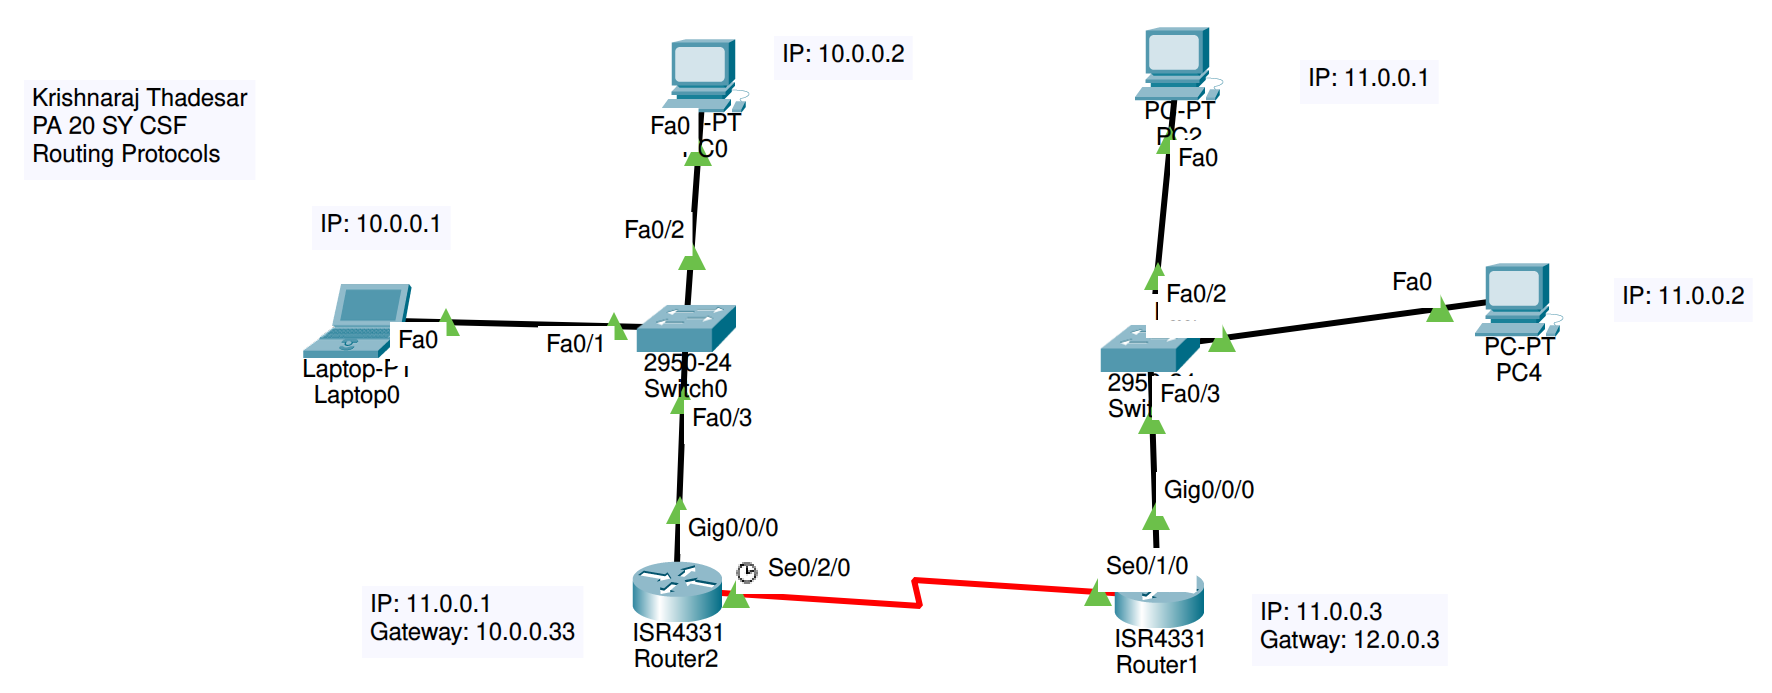
\includegraphics[scale=0.4]{../Screenshots/Assignment_7_screenshot.png}
\end{figure}


\section{Conclusion}
Thus routing Protocols were Executed on a simple LAN, and the connection was verified using the ping command. 3 Routing Protocols were executed successfully. RIP, OSPF and EIGRP. Their Differences were studied and understood. 
\end{document}